%%% LaTeX Template
%%% This template can be used for both articles and reports.
%%%
%%% Copyright: http://www.howtotex.com/
%%% Date: February 2011

%%% Preamble
\documentclass[paper=a4, fontsize=11pt]{scrartcl}	% Article class of KOMA-script with 11pt font and a4 format

\usepackage[english]{babel}
\usepackage[utf8]{inputenc}
\usepackage[protrusion=true,expansion=true]{microtype}				% Better typography
\usepackage{amsmath,amsfonts,amsthm}										% Math packages
\usepackage[pdftex]{graphicx}														% Enable pdflatex
%\usepackage{color,transparent}													% If you use color and/or transparency
\usepackage[hang, small,labelfont=bf,up,textfont=it,up]{caption}	% Custom captions under/above floats
\usepackage{epstopdf}																	% Converts .eps to .pdf
\usepackage{subfig}																		% Subfigures
\usepackage{booktabs}																	% Nicer tables
\usepackage{hyperref}
\usepackage{pdflscape}


%%% Advanced verbatim environment
\usepackage{verbatim}
\usepackage{fancyvrb}
\DefineShortVerb{\|}								% delimiter to display inline verbatim text


%%% Custom sectioning (sectsty package)
\usepackage{sectsty}								% Custom sectioning (see below)
\allsectionsfont{%									% Change font of al section commands
	\usefont{OT1}{bch}{b}{n}%					% bch-b-n: CharterBT-Bold font
%	\hspace{15pt}%									% Uncomment for indentation
	}

\sectionfont{%										% Change font of \section command
	\usefont{OT1}{bch}{b}{n}%					% bch-b-n: CharterBT-Bold font
	\sectionrule{0pt}{0pt}{-5pt}{0.8pt}%	% Horizontal rule below section
	}


%%% Custom headers/footers (fancyhdr package)
\usepackage{fancyhdr}
\pagestyle{fancyplain}
\fancyhead{}														% No page header
\fancyfoot[C]{\thepage}										% Pagenumbering at center of footer
\renewcommand{\headrulewidth}{0pt}				% Remove header underlines
\renewcommand{\footrulewidth}{0pt}				% Remove footer underlines
\setlength{\headheight}{13.6pt}

%%% Equation and float numbering
\numberwithin{equation}{section}															% Equationnumbering: section.eq#
\numberwithin{figure}{section}																% Figurenumbering: section.fig#
\numberwithin{table}{section}																% Tablenumbering: section.tab#


%%% Title
\title{ \vspace{-1in} 	\usefont{OT1}{bch}{b}{n}
		\huge \strut BudgetChef \strut \\
		\Large \bfseries \strut Documentação de Projeto - MAC0332 \strut
}
\author{
				Guilherme Schützer - 8658544\\
				Renato Geh - 8536030\\
				Ricardo Lira - 8536131\\
				Tomás Paim - 7157602\\ \usefont{OT1}{bch}{m}{n}
        Instituto de Matemática e Estatística - USP\\	\usefont{OT1}{bch}{m}{n}
        Departamento de Ciências da Computação\\
}
\date{\today}


%%% Begin document
\begin{document}
\maketitle
\addtocounter{section}{-1}
\section*{Fase 0}

\addtocounter{section}{1}

\subsection{Proposta de projeto}

Criação de um aplicativo mobile para gerenciar os produtos gastronômicos de sua casa, determinar quantidades e avisar sobre datas de validades próximas do vencimento, recomendar receitas que utilizam produtos disponíveis ou determinar o que falta para abastecer seu lar.
\\ \\ Link para o Canvas: \url{https://canvanizer.com/canvas/Jp4RFxBWnoI}

\subsection{Requisitos}

\begin{itemize}

\item Framework para aplicativos móveis e interação web.
\item Banco de dados.
\item \emph{Hardware} e \emph{software}: \emph{smartphone} e servidores de acordo com o número de usuários e de receitas.

\end{itemize}

\subsection{Viabilidade do sistema}

O aplicativo tem um grande escopo de público alvo, cobrindo desde jovens adultos a responsáveis por famílias. A flexibilidade do aplicativo permite que qualquer pessoa que tenha interesse em descobrir novas receitas, seja por necessidade ou por curiosidade, possa ter com facilidade uma receita disponível para se fazer na hora.
\\ \\
Por ser um aplicativo intuitivo e sem custo para o usuário padrão, BudgetChef é acessível a qualquer um que tenha um smartphone compatível com o requerido pelo aplicativo.
\newpage
A interface do aplicativo permite navegar com facilidade por todas as suas funcionalidades. O envio de novas receitas é feito de forma intuitiva e simples, apenas sendo necessário ter uma conta válida, além de o próprio aplicativo ajudar no que se deve adicionar a sua nova receita, sugerindo novas informações conforme o usuário as vai colocando. O aplicativo também sugere receitas que sejam similares àquelas que ele havia pesquisado ou enviado.

\section*{Fase 1}
\addtocounter{section}{1}
\addtocounter{subsection}{-3}


\subsection{Dicionário de Dados}


\subsubsection{} A primeira relação é de receitas. Contém os campos não-multivalorados necessários para descrever uma receita e avaliá-la.


\begin{center}
\begin{tabular}{ l l l l l }
  \multicolumn{5}{l}{\textbf{RECEITAS}} \\
  \hline
  \textbf{Chave} & \textbf{Campo} & \textbf{Descrição} & \textbf{Tipo} & \textbf{Tamanho} \\
  \cline{1-5}
  Primária & REC\_CODIGO & Código da Receita & Inteiro & 8 \emph{bits}  \\
   & REC\_NOME & Nome da Receita & Texto & 255 \\
   & USU\_LOGIN & Usuário autor da Receita & Texto & 255 \\
   & REC\_DATA & Data de Submissão & Data & 6 \\
   & REC\_TEMPO & Tempo de preparo & Tempo(Inteiro) & 4 \\
   & REC\_PORC & Quantas porções serve & Inteiro & 8 \emph{bits} \\
   & REC\_AVAL & Quantidade de avaliações & Inteiro & 8 \emph{bits} \\
   & REC\_MEDIA & Média das avaliações & Decimal & 5,00 \\
   & REC\_VISIT & Quantidade de visitas & Inteiro & 8 \emph{bits}
\end{tabular}
\end{center}

\vfill

\subsubsection{} A relação de Ingredientes se refere aos ingredientes necessários para cada receita. Como cada receita pode ter mais de um ingrediente e cada ingrediente pode estar em mais de uma receita, os dois campos constituem a chave primária.

\begin{center}
\begin{tabular}{ l  l  l  l l }
  \multicolumn{5}{l}{\textbf{INGREDIENTES}} \\
  \hline
  \textbf{Chave} & \textbf{Campo} & \textbf{Descrição} & \textbf{Tipo} & \textbf{Tamanho} \\
  \cline{1-5}
  Primária & REC\_CODIGO & Código da Receita & Inteiro & 8 \emph{bits}  \\
  Primária & ING\_NOME & Nome do Ingrediente & Texto & 255 \\
   & ING\_QUANT & Quantidade necessária & Decimal & 16 \emph{bits} \\
   & ING\_UNI & Unidade (colheres, gramas...) & Texto & 255
\end{tabular}
\end{center}

\newpage

\subsubsection{} Relação de Usuário. Contém as informações básicas e para estatísticas de receitas.

\begin{center}
\begin{tabular}{ l  l  l  l l }
  \multicolumn{5}{l}{\textbf{USUÁRIOS}} \\
  \hline
  \textbf{Chave} & \textbf{Campo} & \textbf{Descrição} & \textbf{Tipo} & \textbf{Tamanho} \\
  \cline{1-5}
   Primária & USU\_LOGIN & Nome de \emph{login} & Texto & 255 \\
   Candidata & USU\_EMAIL & Endereço de \emph{e-mail} do usuário & Texto & 255 \\
   & USU\_NOME & Nome completo do Usuário & Texto & 255 \\
   & USU\_MEDIA & Média de todas as avaliações & Decimal & 5,00 \\
   & USU\_RECS & Número de receitas submetidas & Inteiro & 8 \emph{bits}
\end{tabular}
\end{center}

\vfill

\subsubsection{} Relação de Estoques. Parecida com a relação Ingredientes, mas referente ao estoque de cada usuário e não às receitas. Contém também informações de validade.

\begin{center}
\begin{tabular}{ l  l  l  l l }
  \multicolumn{5}{l}{\textbf{ESTOQUE}} \\
  \hline
  \textbf{Chave} & \textbf{Campo} & \textbf{Descrição} & \textbf{Tipo} & \textbf{Tamanho} \\
  \cline{1-5}
  Primária & USU\_LOGIN & \emph{Login} do Usuário & Texto & 255 \\
  Primária & ING\_NOME & Nome do Ingrediente em estoque & Texto & 255 \\
   & EST\_QUANT & Quantidade em estoque & Decimal & 16 \emph{bits} \\
   & EST\_UNI & Unidade (colheres, gramas...) & Texto & 255 \\
   & EST\_DATA & Data de estocagem & Data & 6 \\
   & EST\_VAL & Data de validade & Data & 6
\end{tabular}
\end{center}

\vfill

\subsubsection{} Relação das Famílias dos Ingredientes. Útil para praticidade de entrada.

\begin{center}
\begin{tabular}{ l  l  l  l l }
  \multicolumn{5}{l}{\textbf{FAMÍLIAS}} \\
  \hline
  \textbf{Chave} & \textbf{Campo} & \textbf{Descrição} & \textbf{Tipo} & \textbf{Tamanho} \\
  \cline{1-5}
  Primária & FAM\_NOME & Nome da Família (carne, carboidrato...) & 255 \\
  Primária & ING\_NOME & Nome do Ingrediente & Texto & 255 \\
  & FAM\_DESC & Breve descrição da Família & Texto & 255
\end{tabular}
\end{center}

\newpage

\subsubsection{} Relação das Categorias das Receitas. Categorias podem ser usadas como filtro na busca de receitas.

\begin{center}
\begin{tabular}{ l  l  l  l l }
  \multicolumn{5}{l}{\textbf{CATEGORIA}} \\
  \hline
  \textbf{Chave} & \textbf{Campo} & \textbf{Descrição} & \textbf{Tipo} & \textbf{Tamanho} \\
  \cline{1-5}
  Primária & ATR\_NOME & Nome do Atributo & Texto & 255 \\
  Primária & REC\_CODIGO & Código da receita com o atributo & Inteiro & 8 \emph{bits} \\
   & ATR\_DESC & Breve descrição do Atributo & Texto & 255
\end{tabular}
\end{center}

\subsubsection{} Relação de amizades; atributo multivalorado.

\begin{center}
\begin{tabular}{ l  l  l  l l }
  \multicolumn{5}{l}{\textbf{AMIZADE}} \\
  \hline
  \textbf{Chave} & \textbf{Campo} & \textbf{Descrição} & \textbf{Tipo} & \textbf{Tamanho} \\
  \cline{1-5}
  Primária & USU\_LOGIN & Login de um usuário & Texto & 255 \\
  Primária & USU\_AMIG & Login de seu amigo & Texto & 255
\end{tabular}
\end{center}

\newpage
\subsection{Casos de Uso}

\begin{figure}[h!]
	\centerline{
	\includegraphics[scale=0.5]{casoUso.png}
	}
\end{figure}

As setas cheias representam o destino dos dados quando há mais de um ator possível que pode enviá-los.

\begin{landscape}
\newpage
\subsection{Diagrama de Atividade}

\begin{figure}[h!]
	\centerline{
	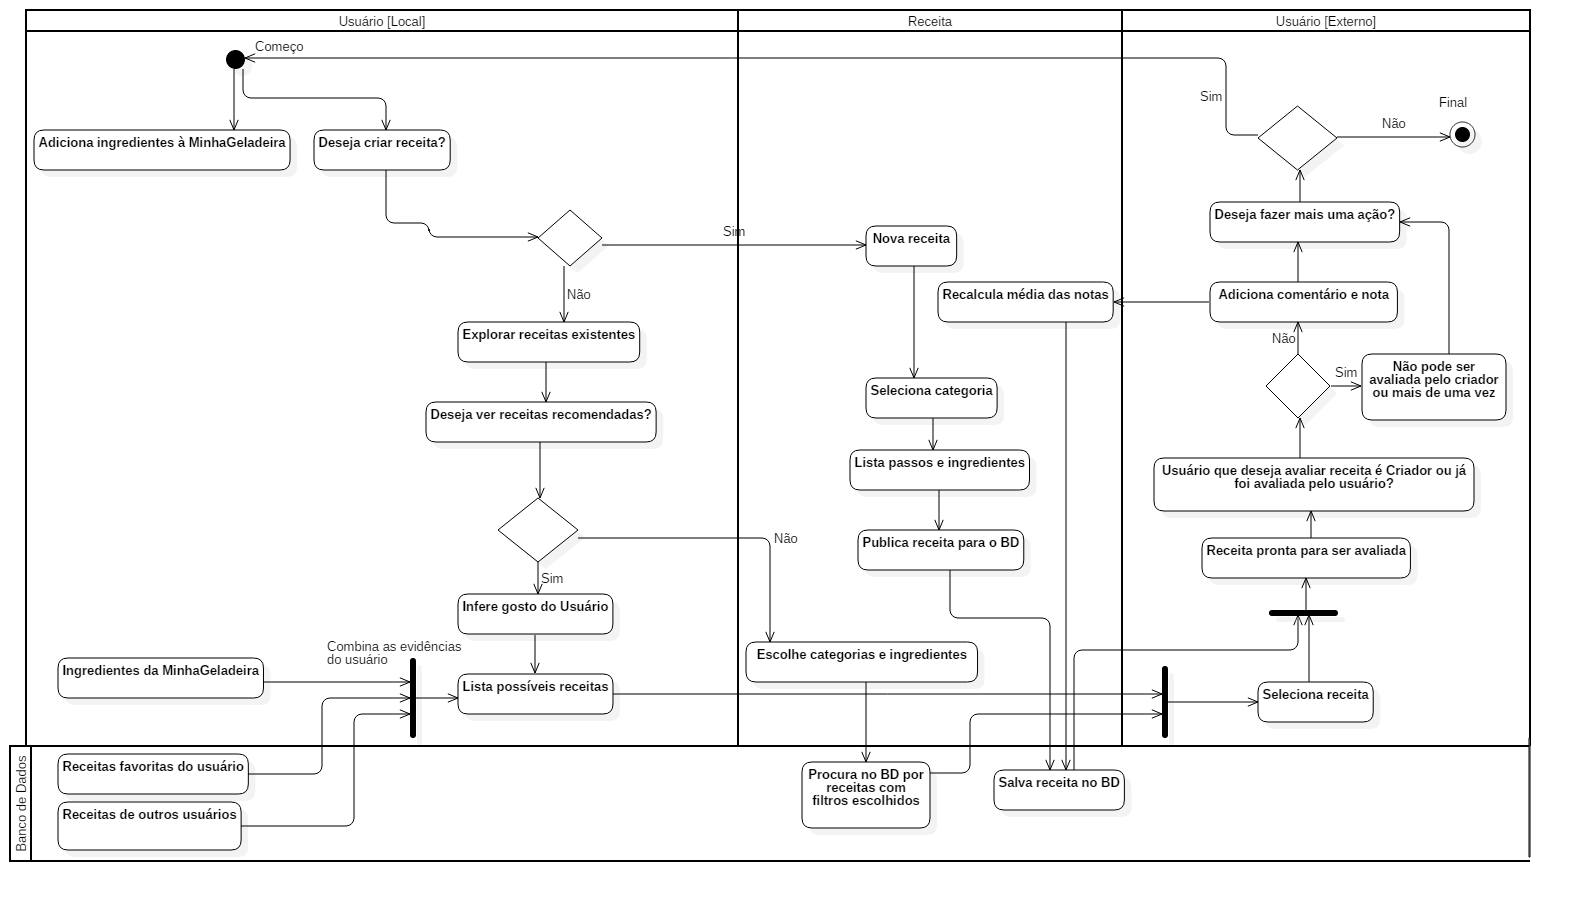
\includegraphics[scale=0.42]{atividade.png}
	}
\end{figure}

\end{landscape}

\newpage
\subsection{Diagrama de Sequência}

\begin{figure}[h!]
	\centerline{
	\includegraphics[scale=0.6]{sequencia.png}
	}
\end{figure}

\newpage
\subsection{Identificação de Objetos/Classes}

\begin{figure}[h!]
	\centerline{
	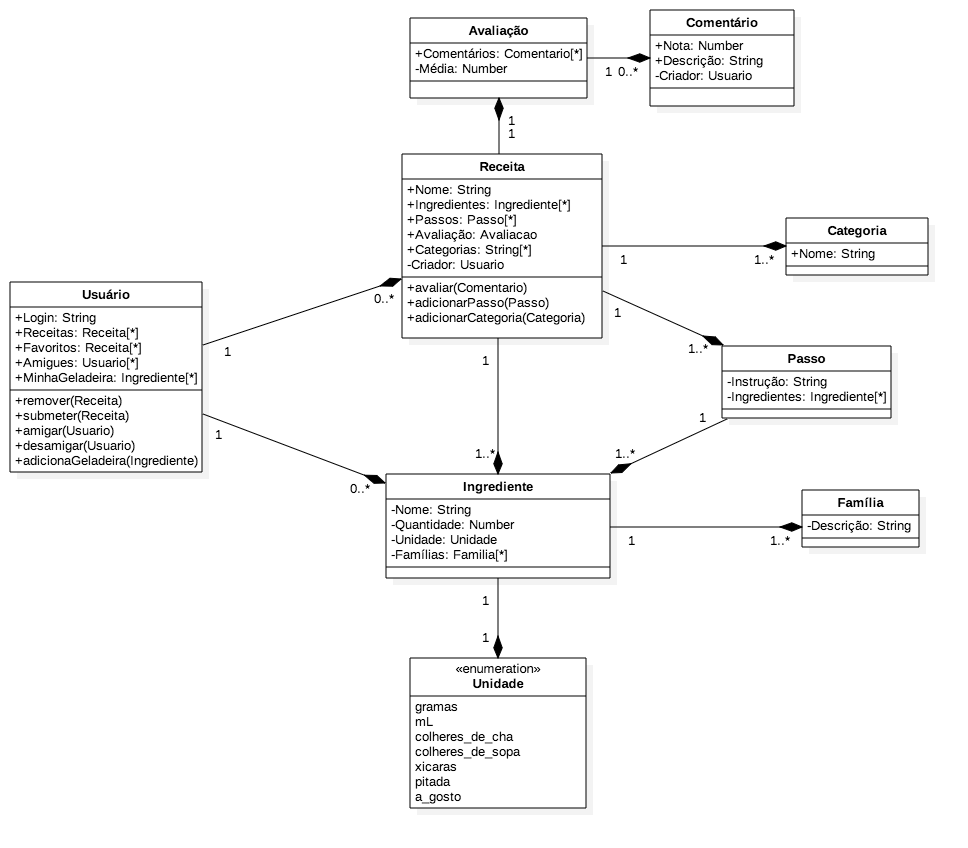
\includegraphics[scale=0.4]{UML.png}
	}
\end{figure}


\newpage
\subsection{Documento de especificação de requisitos}

Julgamos que os requisitos funcionais já estão bem especificados nos diagramas de Caso de Uso e de Atividade. Por esse motivo, listaremos os requisitos não-funcionais.

\begin{center}
\begin{tabular}{l l}
  \textbf{PROPRIEDADE} & \textbf{MÉTRICAS} \\
  \cline{1-2}
	\textbf{Facilidade de uso} & 5 minutos de tutorial são suficientes \\
	\textbf{Portabilidade} & Funcionamento em aparelhos Android™ e iOS™ \\
	\textbf{Segurança} & Uso do \textbf{Internet Protocol Security (IPsec)} \\
	\textbf{Velocidade} & Transferência estável média de 10 KB/segundo \\
	\textbf{Espaço em Disco} & Menos de 100 MB
\end{tabular}
\end{center}





\end{document}
